\addcontentsline{toc}{section}{\hfill[\hei 唱段·唱腔]\hfill}
\chead{唱段·唱腔} % 页眉中间位置内容

\newpage
\phantomsection %实现目录的正确跳转
\section*{{\hei\large 硃痕记~{\small 之}~朱春登}$^{\ast}$}%*
\addcontentsline{toc}{section}{\hei 硃痕记~{\small 之}~朱春登}

\hangafter=1                   %2. 设置从第1⾏之后开始悬挂缩进  %
\setlength{\parindent}{0pt}{
{\centerline{\textrm{{[}\hei 第一场{]}}}}
\vspace{5pt}

\setlength{\hangindent}{56pt}{【{\akai 二黄散板}】听说是老娘黄泉命染,好一似刀割肉箭把心穿。问婶娘她婆媳何处埋掩。叫李仁备祭品\footnote{吴焕老师整理的剧本作``备祭礼''。}%\protect\hyperlink{fn631}{\textsuperscript{631}}
坟前祭奠,我只得身穿孝头戴麻冠。
}

\vspace{3pt}{\centerline{\textrm{{[}{\hei 第二场}{]}}}}\vspace{5pt}

【{\akai 二黄导板}】见坟台不由人泪流满面,

【{\akai 回龙}】尊一声去世娘细听儿言:~

\setlength{\hangindent}{66pt}{   %3. 设置悬挂缩进量                %
【{\akai 反二黄慢板}】都只为西域国黄龙造反,是孩儿替叔父去到军前。抖威风杀贼寇全凭神箭,灭黄龙平西域得胜回还。王封儿平西侯官高爵显,奉圣命回家来祭奠祖先。实指望母子们欢聚团圆,料不想儿的娘命染黄泉。哭老娘把儿的肝肠痛断,肝肠痛断,儿的娘啊,
}

\setlength{\hangindent}{66pt}{   %3. 设置悬挂缩进量                %
【{\akai 反二黄原板}】食什么爵禄做的是什么官。哭罢了老娘亲把妻房呼唤,叫一声贤德妻你在哪边。我和你夫妻情恩爱不浅,撇下我独一人凄凉孤单。哭一声贤德妻难得相见,难得相见,
}

【{\akai 反二黄散板}】要相逢除非是梦里团圆。

\setlength{\hangindent}{56pt}{【{\akai 西皮三眼}】听我妻赵锦棠言讲一遍,好一似刀割肉箭把心攒。婶娘道她婆媳黄泉命染,为什么她还在阳世之间。莫不是她死得苦冤魂不散,莫不是魍魉鬼来把我缠。我这里出席棚用目观看,观只见那红日未落西山。猛想起赵锦棠左手心硃砂红点,是不是真和假向前去细问根源。
}

\textless{}\!{\bfseries\akai 哭头}\!\textgreater{}啊,我的妻呀!

【{\akai 西皮散板}】问贤妻老娘亲何方避难。

【{\akai 西皮散板}】有劳你前引路把母来见,

【{\akai 西皮散板}】儿就是朱春登做官回还。}
   %% 硃痕记
\newpage
\phantomsection %实现目录的正确跳转
\section*{\hei\large 蟠桃会~\protect\footnote{此戏别名《海屋添筹》或《八仙庆寿》,是一出武旦戏。}~%\protect\hyperlink{fn632}{\textsuperscript{632}}
{\small 之}~吕洞宾$^{\ast}$}
\addcontentsline{toc}{section}{\hei 蟠桃会~{\small 之}~吕洞宾}

\hangafter=1                   %2. 设置从第1⾏之后开始悬挂缩进  %
\setlength{\parindent}{0pt}{
{\centerline{{{[}\hei 第一场{]}}}}
\vspace{5pt}

\setlength{\hangindent}{56pt}{【{\akai 西皮原板}】忆昔当年赴科场,科场中提笔做文章。文章幸喜龙颜赏,赏赐我进士伴君王。陪王伴君心不想,一心只想上天堂。天堂就在瑶池上\footnote{此句吴小如先生从刘曾复先生学的是``天堂远在瑶池上''。}%\protect\hyperlink{fn633}{\textsuperscript{633}}
,瑶池以上福寿绵长。}

\vspace{3pt}{\centerline{{{[}{\hei 第二场}{]}}}}\vspace{5pt}

{【{\akai 西皮散板}】离了洞府到仙界,见了众仙说开怀。}

{【{\akai 西皮散板}】瑶池以上寿筵席开。}

\setlength{\hangindent}{56pt}{{【{\akai 西皮原板}】今日里饮酒多爽快,好似仙子({\akai 或}:~好一似黄粱)赴瑶台。这仙女({\akai 或}:~这仙子)生得呀多娇态,眉清目秀送情来。趁此佳兴({\akai 或}:~趁此酒兴)破了戒,}
}

{【{\akai 西皮原板}】众仙道我理不该。将身且坐({\akai 或}:~将身来在)瑶池外,昏昏沉沉睡石台。}

\vspace{3pt}{\centerline{{{[}{\hei 第三场}{]}}}}\vspace{5pt}

{【{\akai 西皮导板}】沉醉东风}\footnote{樊剑{\scriptsize 君}此处建议作``沉醉洞府''。}%\protect\hyperlink{fn634}{\textsuperscript{634}}
{月儿高,}

\setlength{\hangindent}{56pt}{{【{\akai 西皮原板}】忆昔当初饮酕醄。两足徘徊任颠倒,湘子、仙姑发笑嘲。你道我当真吃醉了,任意随心乐逍遥。游戏三昧多奥妙,}
}

\setlength{\hangindent}{56pt}{【{\akai 西皮快板}】坎离\footnote{八卦中
``坎''(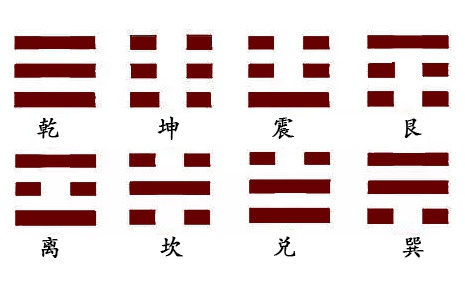
\includegraphics[height=9t,width=9pt, viewport=120 59 225 140,clip]{Eight_Gua.jpeg})为水,
``离''(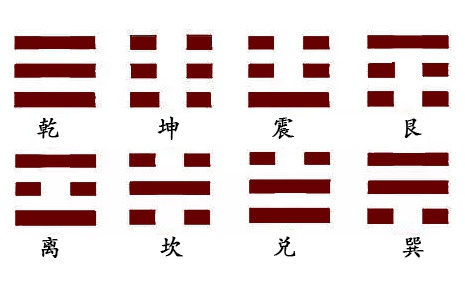
\includegraphics[height=9pt,width=9pt, viewport=5 59 100 140,clip]{Eight_Gua.jpeg})为火。此处寓为``水火既济''之意。}%\protect\hyperlink{fn635}{\textsuperscript{635}}
二字本相调。不觉来到东海道,海水接天浪滔滔。}

{【{\akai 西皮散板}】宝剑扔在东海道,你看我醉仙家的道法高不高?}

{【{\akai 西皮散板}】柳仙带路东海道,万丈波涛走一遭。}

{【{\akai 西皮散板}】湘子说话不中听,丢了宝贝你问旁人。}

{【{\akai 西皮散板}】洞宾主意拿得稳,从今后不管闲事情。}

(李铁拐\hspace{20pt}【{\akai 西皮散板}】$\cdots${}$\cdots${}{入东海道,)}

{【{\akai 西皮散板}】从今后戒酒最为高。}
}
   %% 蟠桃会
\newpage
\subsubsection{\hei\large 霸王别姬·山头~{\small 之}~ 韩信$^{\ast}$}
\addcontentsline{toc}{subsection}{\hei 霸王别姬~{\small 之}~韩信}

\hangafter=1                   %2. 设置从第1⾏之后开始悬挂缩进  %
\setlength{\parindent}{0pt}{

\setlength{\hangindent}{65pt}{   %3. 设置悬挂缩进量                %
\textrm{【{\akai 西皮散板}】李左车引霸王入了阵道,众诸侯齐奋勇争立功劳。直杀得血成河尸如山倒,灭西楚擒霸王就在今朝。}
}

\setlength{\hangindent}{65pt}{   %3. 设置悬挂缩进量                %
\textrm{【{\akai 西皮散板}】传一令犹如那泰山压倒,兵将涌如那海水临潮。楚项羽犹如那无翼之鸟,失彭城犹如那猛虎离巢。}
}

\setlength{\hangindent}{65pt}{   %3. 设置悬挂缩进量                %
\textrm{【{\akai 西皮散板}】直杀得楚项羽人喊马叫,直杀得子弟兵四路奔逃。直杀得天昏暗日无光耀,直杀得夜更深月挂松梢。}
}

\textrm{(项羽\hspace{25pt}~ 【{\akai 西皮散板}】越杀越勇心焦躁,)}

\textrm{【{\akai 西皮散板}】三军带马回营道,请出张良作计较。}
}
   %% 霸王别姬·山头
\newpage
\phantomsection %实现目录的正确跳转
\section*{\hei\large 逍遥津~{\small 之}~汉献帝$^{\ast}$}
\addcontentsline{toc}{section}{\hei 逍遥津~{\small 之}~汉献帝}

\hangafter=1                   %2. 设置从第1⾏之后开始悬挂缩进  %
\setlength{\parindent}{0pt}{

【{\akai 二黄导板}】苦汉帝在后宫伤心难忍,

【{\akai 回龙}】父子们悲切切好不伤情,贤御妻呀。

\setlength{\hangindent}{52pt}{   %3. 设置悬挂缩进量                %
【{\akai 二黄原板}】叹伏后此时间必定丧命,我君妃生离散惨不忍闻。二皇儿年幼小孩童天性,哭啼啼与孤王要他的娘亲。想奸贼不由孤咬牙愤恨,上欺寡人下压群臣。欺寡人贼带剑上殿孤见他不敢责问,欺寡人贼独霸朝纲、目无君王、自专自尊。欺寡人孤只得百般谨慎,欺寡人孤只得时刻留心。欺寡人贼奏本是非曲直孤不敢争论,欺寡人孤有命贼大胆妄为抗旨不遵。欺寡人贼一意孤行孤不敢过问,欺寡人孤怒不敢言、忍耐在心。欺寡人孤见他气色不正吓得孤乱了方寸,欺寡人孤见他带怒发威吓得孤胆战心惊。欺寡人蹂躏百般、万分难忍,欺寡人贼败坏朝纲、逆了五伦。欺寡人好一似【{\footnotesize 转}{\akai 二黄慢板}】奴仆受训,欺寡人好一似虐待家人。欺寡人好一似无辜良民被贼围困,欺寡人好一似冤屈罪犯无处冤申。欺寡人好一似蛇毒蝎狠,欺寡人好一似虎咽狼吞。欺寡人好一似前世冤孽今生报应,欺寡人好一似狭路相逢对头仇人。欺寡人好一似阎君索命,欺寡人好一似饿鬼孤魂。欺寡人好一似败阵残兵无投奔,反被贼困垓心难逃遁难存身,坐以待毙谁来救应,
}

【{\akai 二黄散板}】又听得一片喧哗声震乾坤。}

\vspace{15pt}
{\hei 附注}:~

\setlength{\parindent}{0pt}{
《顺天时报》曾刊《逍遥津任辰辙之唱词》一文,所载词句与刘曾复先生所传词句非常相近,照录供参考(张斯琦{\scriptsize 君}提供)
}

\vspace{10pt}
{\centerline{\textcolor{blue}{\hei《逍遥津》``任辰''辙之唱词}}}
\vspace{10pt}

\setlength{\parindent}{22pt}{     %
	{\hwfs 旧本《逍遥津》,``欺寡人''一段,俱用``由求''辙,戏中汉献帝唱``欺寡人好一比鹰抓兔胁''句,过于俚俗,殊伤大雅。刘鸿升未故时,将``由求''改``任辰'',虽亦不免俗,但较旧本,似觉雅驯。李桂芬唱《逍遥津》,亦用斯词,爰将改词录于左端:~}}

\vspace{15pt}
\setlength{\parindent}{0pt}{
	{\hei 汉献帝在后宫伤心难忍,可叹我父子们悲切切冷清清、求生不得求死不能、好不惨情。叹伏后到此时难保活命,我君妃生离散惨不忍闻。二皇儿年幼小孩童之性,哭啼啼与孤王要他的娘亲。想奸贼不由孤嚼牙愤恨,上欺天子下压群臣。欺寡人(贼)带剑上殿孤见他不敢责问,欺寡人(贼)独霸朝纲、目无君、自耑自尊。欺寡人孤只得百般谨慎,欺寡人孤只得时刻留神。欺寡人(贼)奏本是非曲直孤不敢\textcolor{red}{$\square~\square$},欺寡人孤有命贼大胆妄为抗旨不遵。欺寡人贼自由行孤不敢过问,欺寡人孤怒不敢言、忍耐在心。欺寡人孤见他气色不正嚇得孤乱了方寸,欺寡人孤见他怒发威嚇得吊胆提心。欺寡人蹂躏百般、惨忍万分,欺寡人贼败坏纲常、逆了五伦。欺寡人好一似主仆受训,欺寡人好一似虐待家人。欺寡人好一似无辜良民被贼围困,欺寡人好一似冤屈罪犯\textcolor{red}{$\square$}而受刑。欺寡人好一似蛇毒蝎狠,欺寡人好一似虎狼把孤吞。欺寡人好一似前世冤孽今生报应,欺寡人好一似夹路相逢对头仇人。欺寡人好一似阎王索命,欺寡人好一似饿鬼勾魂。欺寡人好一似败阵惨兵无投奔,反被贼困垓心、难逃命、难生存、认贼斩、恁贼擒,孤做一待毙谁来救应,又听得宫门外喧哗之声。
}}
   %% 逍遥津
